\documentclass[10pt]{extarticle} % article doctype, possible font size range from 8pt to 20pt with not all being avaiable.
\setcounter{secnumdepth}{4} % Max. section depth, e.g. 3 means 4.1.1 is possible but not 4.1.1.2
\title{\huge Technical Design Document MaramaUU}
\author{Tim Hintzbergen, Wilbert Schepenaar, <nextname>    \\s1097561, s1094484, <nextcode>
\\\\ICTGPb
\\Wilco Moerman}
\date{May 8th, 2018 <TODO>}

% include packages
\usepackage{graphicx}
\usepackage{caption}
\usepackage{mathabx}
\usepackage[margin=1.0in]{geometry} % Sets page margin, 2.0in is default.
\usepackage{titlesec}
\usepackage{hyperref}

% custom commands
\newcommand{\myparagraph}[1]{\paragraph{#1}\mbox{}\\} % Without \mbox{} all newlines will be ignored, making the first sentence appear on the same line as a paragraph title.

\DeclareCaptionFormat{cancaption}{#1#2#3\par} % Normal format actually
\DeclareCaptionLabelFormat{cancaptionlabel}{#1}
\captionsetup[figure][number]{format=cancaption,labelformat=cancaptionlabel}
\graphicspath { {images/} }
\begin{document}
    \maketitle
    \thispagestyle{empty}
    \newpage
    %------------------------------------------------------------------------------------------------------------------------------------------------------- Introduction
    \newpage
    \setcounter{page}{1}
    \section {Introduction}
    This document contains all technical aspects of the product.
    It describes the requirements, the architecture, the design choices and the epics.
    The requirements talk about all functional and non-functional requirements of the product.
    The architecture explains the form of the product, offers a clear overview and talks about some minute details.
    The list of design choices illustrates and defend the various choices that have been made during the design and construction of the product.
    Finally the epics list all coherent components of the product and their submodules
    \newpage

    \tableofcontents{}
    \newpage

    %------------------------------------------------------------------------------------------------------------------------------------------------------- Requirements
    \section{Requirements}
    Functional and Non-functional requirements.
    \newpage

    %------------------------------------------------------------------------------------------------------------------------------------------------------- Architecture
    \section{Architecture}
    A high-level overview of the architecture of the system.
    A UML component diagram can give a clear overview.
    Boxes and arrows can be used during an early stage of the design.
    It should be clear where different techniques (programming languages, database systems, data formats, frameworks, ..) are used in the system.
    Class diagrams and package diagrams for the different components of your system.
    Subdivide class diagrams into smaller diagrams that focus on a particular aspect.
    Think about which details can be left out (e.g.\ private attributes and methods).
    Always make sure diagrams are readable when printed on paper.
    Only provide a textual description of classes and methods that require additional explanation.
    \item \begin{itemize}
              \item Sequence diagrams to show interactions between objects, if the interaction is particularly complex or involves many objects.
              \item Deployment diagrams to show the hardware and middleware on which the different software components run.
              \item Database designs, such as ERD diagrams.
              \item Descriptions of custom protocols, data formats etc.
              \item Security measures and considerations.
              \item Algorithm designs.
    \end{itemize}

    \subsection[class_diagram]{Class diagram}

    Database designs, such as ERD diagrams.

    Descriptions of custom protocols, data formats etc.

    Security measures and considerations.

    Algorithm designs.

    \subsection{Project Structure}
    LibGDX enforces a certain project structure\cite{libgdxprojstruct}.
    The project root directory contains subdirectories for each different target system. (e.g. android, ios, desktop)
    These directories contain specifics for each different target and also acts as entry point for that target to our product.
    Furthermore there is the core directory which contains the actually source and business logic of our product.
    Next up is the documentation directory which, together with a local auxil directory make up our documentation, using \LaTeX\ of course.
    Finally there are a couple of build and property files together with the gitignore file.


    In the below diagram the core functionality of the entire Marama-View is described.\\
    This will be followed with an explanation of the different parts of this diagram for instance the LibGDX and the Screens part. \\
    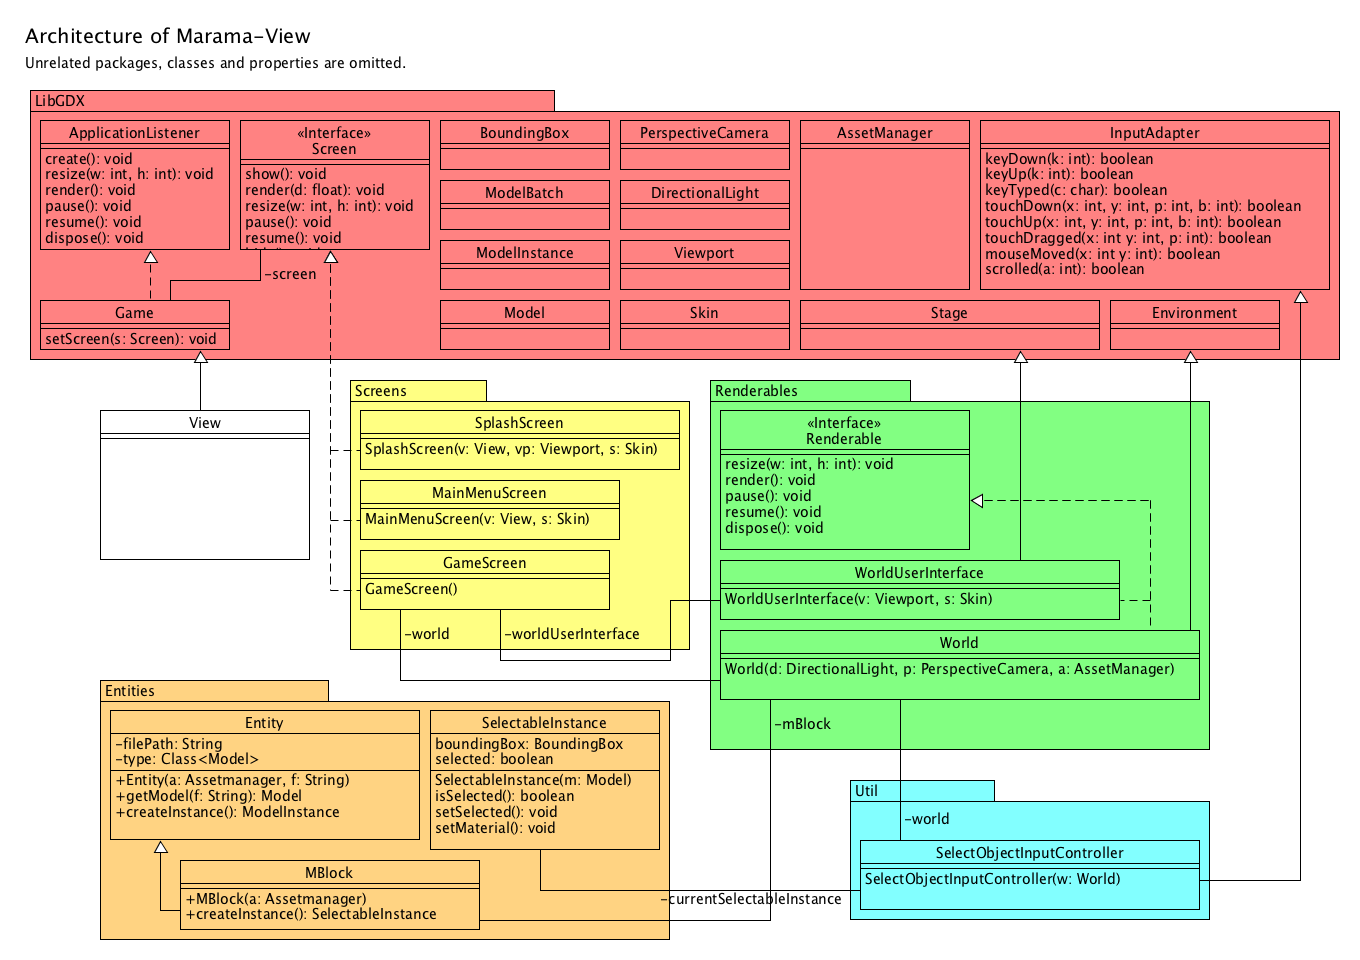
\includegraphics[width=1\linewidth]{architecture-marama-view.png}

    \emph{Some class diagram description} \\
    \subsubsection[LibGDX]{LibGDX}
    The red part of the class diagram contains the LibGDX library.
    As you can see, even though not every line is drawn (so the diagram is way clearer), LibGDX is used a lot.
    Many already existing classes are extended or used.
    This is done because on one side, we shouldn't write any code or build a structure that's already been thought of or worked out.
    On the other side the LibGDX library really fits our own perspective of what the structure of the application should be.
    Due to this, using the library happens pretty naturally and doesn't require much research.


    \newpage

    %------------------------------------------------------------------------------------------------------------------------------------------------------- Design Choices
    \section{Design Choices}
    Design decisions: discuss the motivation (arguments/reasons), consequences,
    and alternatives for the decisions.
    Onderverdeeld in epics ipv user stories, makkelijker te snappen, overzichtelijker, etc. beschrijven..

    Description of custom protocols, data formats etc.\\
    Security measures and considerations.\\
    Coding conventions may be added (as appendix).\\
    Diagrams need textual explanation of context, interpretation and underlying design decisions and reasoning.\\

    It has been decided to resizes texture assets to dimensions in the power of two.
    This is to maintain backwards compatibility for OpenGL ES 1.0, to keep all functionality (some libGDX features are otherwise not supported) and it is a bit more memory efficient.\cite{libgdxpottex}

    \subsection{Epics}
    The view is made up of different epics.
    Epics are a collection of user stories that share a goal or functionality.

    \newcommand{\clickup}[1]{https://app.clickup.com/757520/761304/t/#1}

    \subsubsection{3D Camera Controls}
    \myparagraph{\href{\clickup{2e2ca}}{\#2e2ca} As a MGD or player I want to zoom in/out on the world when pinching}
    The camera zoom functionality is already implemented and enabled by libGDX on all supported devices (Desktop, Android).
    \myparagraph{\href{\clickup{2e2c1}}{\#2e2c1} As a MGD or player I want to rotate the camera by one-fingered swiping}
    The camera rotation functionality is already implemented and enabled by libGDX on all supported devices (Desktop, Android).

    \subsubsection{UI}
    \myparagraph{\href{\clickup{302qb}}{\#302qb} As a user I want to see the Marama logo on start-up}
    When the program is started, independent of which built is used, the splashscreen is displayed first.
    The splashscreen displays the marama-logo and fades out and finally transitions into the mainmenu.
    The fade-out time and total duration are variable and can be changed by changing their respective constants in the SplashScreen.java file.

    \myparagraph{Early sketch of the interface}
    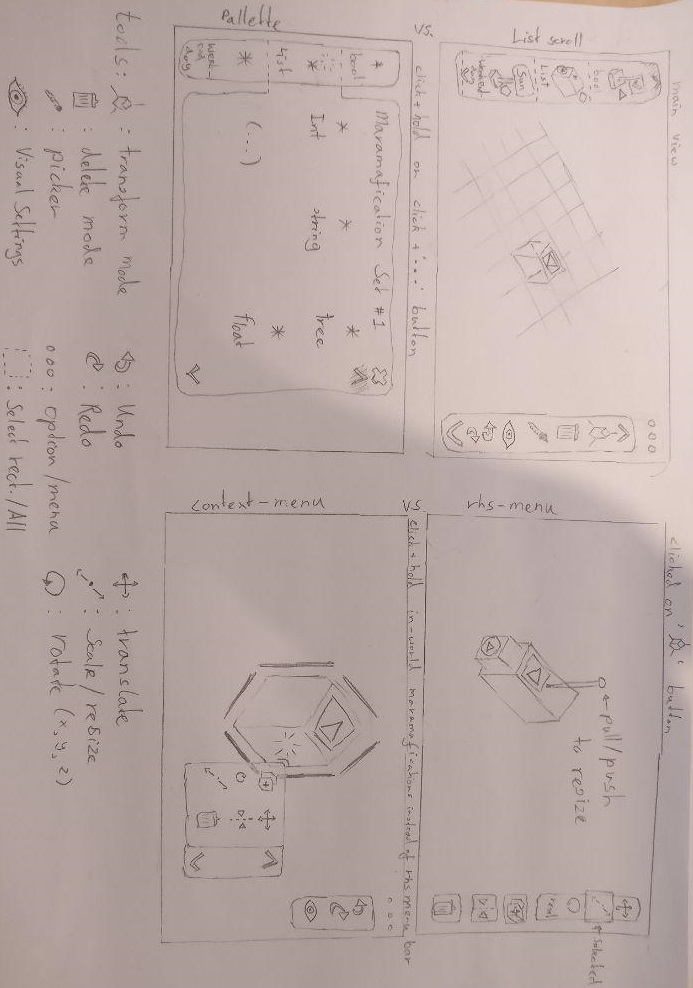
\includegraphics[width=1\linewidth]{marama-view-sketch.jpg}
    This sketch describes two pairs of different interfaces for the editor.
    The first pair shows different approaches to 'a pallette of maramafication'.
    The first one includes a scrollable list and the second one includes a (non-scrollable) pallette which the user can fill with the maramafication he or she needs at the moment.
    The second pair displays several ways to interact with an M-block in the editor.
    TODO
    The interface design is inspired by a 3D sandbox app for android.\thanks{https://play.google.com/store/apps/details?id=com.octagonstudio.assemblr}

    \subsubsection{3D Object Controls}
    \myparagraph{\href{\clickup{2e29e}}{\#2e29e} As a MGD or player I want to be able to select a 3D object}
    Eventually, the user of the editor needs functionality for manipulating 3D objects.
    This means moving, rotating and deleting 3D objects in and from the editor.
    Before any manipulation can occur, the user needs to be able to select 3D objects that are rendered inside the editor.
    A common way for selecting objects in a 3D world is to add some sort of click functionality.
    When the user clicks on a 3D object that is rendered in the editor, the 3D object will be marked as selected.
    The selected object must be properly highlighted so the user knows which object is selected.

    Before a 3D object is able to be selected, the object needs to implement a BoundingBox.
    A BoundingBox can be calculated from a rendered 3D Object and can be seen as a rectangular box.
    This box is able to determine whether it is intersected by a ray.
    Rays can be seen as lasers that can be fired from and to a certain location in the World.
    The ray will be casted from the origin of the camera by the user when he/she clicks on the screen.
    The first BoundingBox that is intersected by the ray will be the selected object.
    Casting the rays from the camera origin and locating the first intersected BoundingBox will prevent that 3D objects in the background are selected.

    \newpage
    %------------------------------------------------------------------------------------------------------------------------------------------------------- Build Automation
    \section{Continous Intergration}
    In this section build automation and its constituent components will be discussed.
    How we applied it, the softwere used and the targets and platforms supported are among a few.

    \newpage
    %------------------------------------------------------------------------------------------------------------------------------------------------------- References
    \bibliography{references}
    \bibliographystyle{ieeetr} % options: apalike for apa, ieeetr for ieee
\end{document}